%! Author = aybehrouz


\subsection{Memory Dependency Graph}\label{subsec:memory-dependency-graph}

Every block of the Argennon blockchain contains a list of transactions. This list is an ordered list and the
effect of its contained transactions must be applied to the AVM state sequentially as they appear in the ordered
list. This ordering is solely chosen by the block proposer, and users should not have any assumptions about
the ordering of transactions in a block.

The fact that block transactions constitute a sequential list, does not mean they can not be executed and applied
to the AVM state concurrently. Many transactions are actually independent and the order of their execution does not
matter. These transactions can be safely validated in parallel by validators.

A transaction can change the AVM state by modifying either the code area or the AVM heap. In Argennon, all
transactions declare the list of memory locations they want to read or write. This will enable us to determine the
independent sets of transactions which can be executed in parallel. To do so, we define the \emph{memory dependency
graph} \(G_d\) as follows:

\begin{itemize}
    \item \(G_d\) is an undirected graph.
    \item Every vertex in \(G_d\) corresponds to a transaction and vice versa.
    \item Vertices \(u\) and \(v\) are adjacent in \(G_d\) if and only if \(u\) has a memory location \(L\) in its
    writing list and \(v\) has \(L\) in either its writing list or its reading list.
\end{itemize}

If we consider a proper vertex coloring of \(G_d\), every color class will give us an independent set of
transactions which can be executed concurrently. To achieve the highest parallelization, we need to color \(G_d\)
with minimum number of colors. Thus, the \emph{chromatic number} of the memory dependency graph shows how good a
transaction set could be run concurrently.

Graph coloring is computationally NP-hard. However, in our use case we don't need to necessarily find an optimal
solution. An approximate greedy algorithm will perform well enough in most circumstances.

After constructing the memory dependency graph, we can use it to construct the
\emph{execution DAG} of transactions. The execution DAG of transaction set \(T\) is a directed acyclic
graph \(G_e = (V_e,E_e)\) which has the \emph{execution invariance} property:
\begin{itemize}
    \item Every vertex in \(V_e\) corresponds to a transaction in \(T\) and vice versa.
    \item Executing the transactions of \(T\) in any order that \emph{respects} \(G_e\) will result in
    the same AVM state.
    \begin{itemize}
        \item An ordering of transactions of \(T\) respects \(G_e\) if for every directed edge \((u,v) \in E_e\)
        the transaction \(u\) comes before the transaction \(v\) in the ordering.
    \end{itemize}
\end{itemize}

Having the execution DAG of a set of transactions, using Algorithm~\ref{alg:exec_dag}, we can apply the transaction
set to the AVM state concurrently, using multiple processor, while we can be sure that the resulted AVM state will
always be the same no matter how many processor we have used.

%##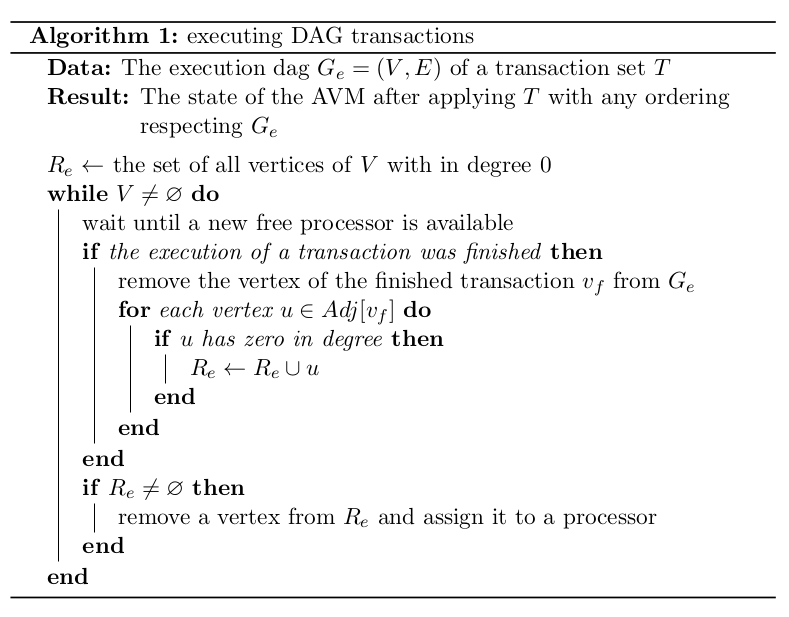
\includegraphics[width=17cm]{../img/Alg1s.png}
\begin{algorithm}
    \DontPrintSemicolon
    \SetKwData{Ready}{$R_e$}\SetKwData{V}{$v_f$}\SetKwData{Graph}{$G_e$}\SetKwData{Vertices}{$V$}\SetKwData
    {Txns}{$T$}
    \KwData{The execution dag $\Graph = (\Vertices,E)$ of transaction set \Txns}
    \KwResult{The state of the AVM after applying \Txns with any ordering respecting \Graph}
    \BlankLine
    \Ready $\gets$ the set of all vertices of \Vertices with in degree 0\;
    \While{$\Vertices \neq \varnothing$}
    {
        wait until a new free processor is available\;
        \If{the execution of a transaction was finished}
        {
            remove the vertex of the finished transaction \V from \Graph\;
            \For{each vertex $u \in Adj[\V]$}
            {
                \If{$u$ has zero in degree}
                {
                    $\Ready \gets \Ready \cup u$\;
                }
            }
        }
        \If{$\Ready \neq \varnothing$}
        {
            remove a vertex from \Ready and assign it to a processor\;
        }
    }
    \caption{executing DAG transactions}\label{alg:exec_dag}
\end{algorithm}

By replacing every undirected edge of a memory dependency graph with a directed edge in such a way that the
resulted graph has no cycles, we will obtain a valid execution DAG. Thus, from a memory dependency graph different
execution DAGs can be constructed with different levels of parallelization ability.

If we assume that we have unlimited number of processors and all transactions take equal time for executing, it
can be shown that by providing a minimal graph coloring to Algorithm~\ref{alg:gen_dag} as input, the resulted
DAG will be optimal, in the sense that it results in the minimum overall execution time.

%##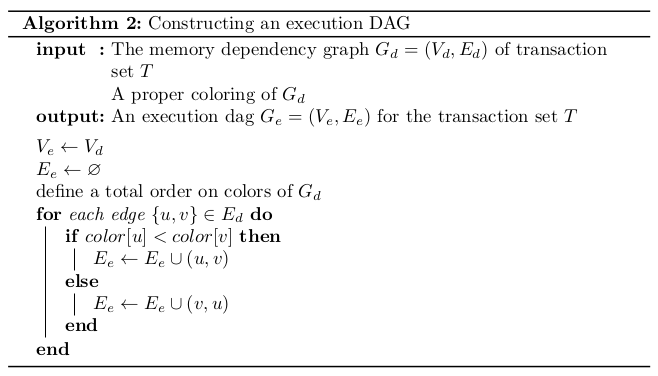
\includegraphics[width=17cm]{../img/Alg2s.png}
\begin{algorithm}
    \DontPrintSemicolon
    \SetKwData{Txns}{$T$}\SetKwData{Gd}{$G_d=(V_d,E_d)$}
    \SetKwInOut{Input}{input}\SetKwInOut{Output}{output}
    \Input{The memory dependency graph \Gd of transaction set \Txns\\A proper coloring of $G_d$}
    \Output{An execution dag $G_e=(V_e,E_e)$ for the transaction set \Txns}
    \BlankLine
    $V_e \gets V_d$\;
    $E_e \gets \varnothing$\;
    define a total order on colors of $G_d$\;
    \For{each edge $\{u,v\} \in E_d$}
    {
        \eIf{$color[u] < color[v]$}
        {
            $E_e \gets E_e \cup (u,v)$\;
        }{
            $E_e \gets E_e \cup (v,u)$\;
        }
    }
    \caption{Constructing an execution DAG}\label{alg:gen_dag}
\end{algorithm}

The block proposer is responsible for proposing an efficient execution DAG alongside his proposed block. This
execution DAG will determine the ordering of block transactions and help validators to validate transactions in
parallel. Since with better parallelization a block can contain more transactions, a proposer is incentivized enough
to find a good execution DAG for transactions.

\subsection{Memory Spooling}\label{subsec:spooling}

When two transactions are dependant and they are connected with an edge \((u,v)\) in the execution DAG,
the transaction \(u\) needs to be run before the transaction \(v\). However, if \(v\) does not read any
memory locations that \(u\) modifies, we can run \(u\) and \(v\) in parallel. We just need to make sure
\(u\) does not see any changes \(v\) is making in AVM memory. This can be done by appropriate versioning
of the memory locations which is shared between \(u\) and \(v\). We call this method \emph{memory spooling}.
After enabling memory spooling between two transactions the edge connecting them can be safely removed from the
execution DAG\@.

\subsection{Concurrent Counters}\label{subsec:concurrent-counters}

We know that in Argennon every transaction needs to transfer its proposed fee to the \texttt{feeSink} accounts
first. This essentially makes every transaction a reader and a writer of the memory locations which store the
balance record of the \texttt{feeSink} accounts. As a result, all transactions in Argennon will be dependant and
parallelism will be completely impossible. Actually, any account that is highly active, for example the account
of an exchange or a payment processor, could become a concurrency bottleneck in our system which makes all
transactions interacting with them dependant.

This problem can be easily solved by using a concurrent counter for storing the balance record of this type of
accounts. A concurrent counter is a data structure which improves concurrency by using multiple memory locations for
storing a single counter. The value of the concurrent counter is equal to the sum of its sub counters and it can
be incremented or decremented by incrementing/decrementing any of the sub counters. This way, a concurrent
counter trades concurrency with memory usage.

Algorithm~\ref{alg:CC} implements a concurrent counter which returns an error when the value of the counter
becomes negative.

%##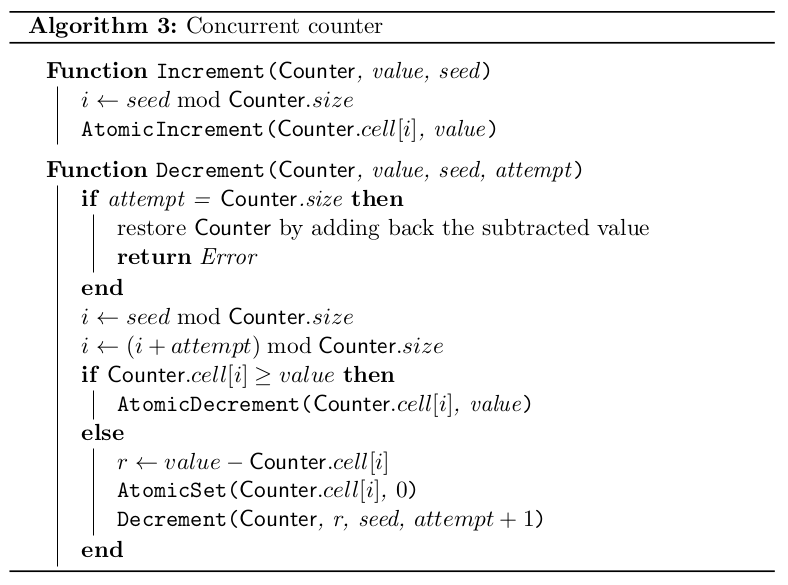
\includegraphics[width=17cm]{../img/Alg3s.png}
\begin{algorithm}
    \DontPrintSemicolon
    \SetKwData{CC}{Counter}
    \SetKwFunction{Inc}{Increment}\SetKwFunction{Dec}{Decrement}\SetKwFunction{AtomInc}{AtomicIncrement}
    \SetKwFunction{AtomDec}{AtomicDecrement}\SetKwFunction{AtomSet}{AtomicSet}\SetKwFunction{Get}{GetValue}
    \SetKwFunction{Acquire}{Lock.Acquire}\SetKwFunction{Release}{Lock.Release}
    \SetKwProg{Fn}{Function}{}{}
    \Fn{\Get{\CC}}
    {
        $s \gets 0$\;
    \Acquire{}\;
    \For{$i \gets 0$ \KwTo $\CC.size - 1$}
    {
        $s \gets s + \CC.cell[i]$\;
    }
    \Release{}\;
    \KwRet{s}\;
    }
    \BlankLine
    \Fn{\Inc{\CC, value, seed}}
    {
        $i \gets seed \bmod \CC.size$\;
    \AtomInc{$\CC.cell[i]$, value}\;
    }
    \BlankLine
    \Fn{\Dec{\CC, value, seed, attempt}}
    {
        \If {attempt = \CC.size}
        {
            restore \CC by adding back the subtracted value\;
            \KwRet{Error}\;
        }
        $i \gets seed \bmod \CC.size$\;
        $i \gets (i + attempt) \bmod \CC.size$\;
    \eIf {$\CC.cell[i] \geq value$}
    {
        \AtomDec{$\CC.cell[i]$, value}\;
    }{
        $r \gets value - \CC.cell[i]$\;
        \AtomSet{$\CC.cell[i]$, $0$}\;
        \Dec{\CC, r, seed, $attempt + 1$}\;
    }
    }
    \caption{Concurrent counter}\label{alg:CC}
\end{algorithm}

It should be noted that in a blockchain application we don't have concurrent threads and therefore we don't need
atomic functions. For usage in a smart contract, the atomic functions of this pseudocode can be implemented like
normal functions.

Concurrent counter data structure is a part of the AVM standard library, and any smart contract can use this data
structure for storing the balance record of highly active accounts.

\subsection{Memory Chunks}\label{subsec:memory-chunks}

In order to further increase the concurrency level of Argennon, we can divide the AVM memory into \emph{chunks}.
Each memory chunk can be persisted using a different ZK-EDB, hence having its own commitment. Then, the
consensus on new values of the commitment of any chunk can be achieved by a different voting committee.

If a transaction does not modify a memory chunk and in the transaction ordering of the block it comes after
any transaction which modifies that chunk, then the execution of that transaction is not needed for calculating
the new commitment of the chunk. Consequently, the voting committee of that memory chunk can safely ignore such a
transaction. The execution DAG of transactions can be used for finding and pruning these transactions as
we see in Algorithm~\ref{alg:prune_dag}.

%##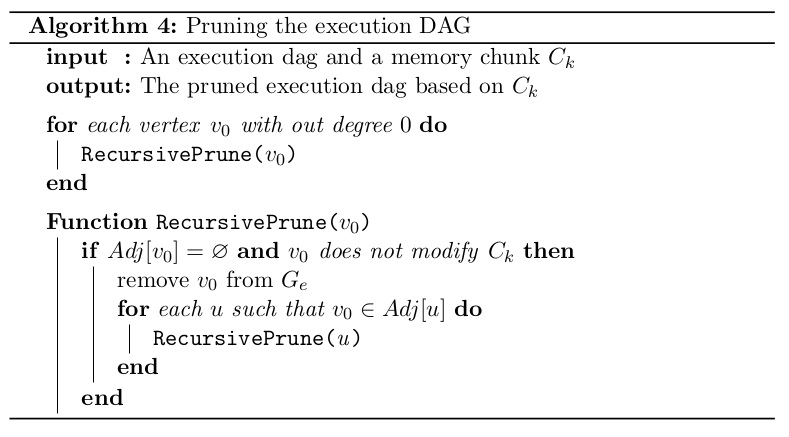
\includegraphics[width=17cm]{../img/Alg4s.png}
\begin{algorithm}
    \DontPrintSemicolon
    \SetKwData{V}{$v_0$}\SetKwData{Graph}{$G_e$}\SetKwData{Chunk}{$C_k$}\SetKwData{Txns}{$T$}
    \SetKwFunction{RPrune}{RecursivePrune}
    \SetKwProg{Fn}{Function}{}{}
    \SetKwInOut{Input}{input}\SetKwInOut{Output}{output}
    \Input{An execution dag \Graph and a memory chunk \Chunk}
    \Output{The pruned execution dag based on \Chunk}
    \BlankLine
    \For{each vertex \V with out degree $0$}
    {
        \RPrune{\V}\;
    }
    \BlankLine
    \Fn{\RPrune{\V}}
    {
        \If{$Adj[\V] = \varnothing$ {\bf and} \V does not modify \Chunk}
        {
            remove \V from \Graph\;
            \For{each $u$ such that edge $(u,\V)$ was in \Graph}
            {
                \RPrune{u}\;
            }
        }
    }
    \caption{Pruning an execution DAG}\label{alg:prune_dag}
\end{algorithm}

If we choose chunks in a way that most transactions only modify memory locations of one chunk,
likely many transactions of a block only need to be validated by one voting committee and can be validated in
parallel by different committees.

Because the voting committees are selected by random sampling, by choosing large enough samples we can make sure
that having multiple voting committees will not change the security properties of the Argennon agreement protocol.